The aim of this chapter is to review key concepts to make the rest of this monograph more easily accessible to computability theorists, set theorists, and combinatorialists. Our terminology and notation will for the most part be standard, following, e.g., \cite{Downey2010Algorithmic} and \cite{Todorcevic2010Ramsey}. Where there is less uniformity in the literature, we highlight our particular usage in this chapter and, as the need arises, in the sequel. In \Cref{sec:bkg_strings} we set out our notation for finite strings, operations on them, and spaces of subsets of $\NN$, which are largely common across these fields. \Cref{sec:bkg_comp,sec:bkg_rm} provide an overview of some technical notions from computability theory and reverse mathematics. In \Cref{sec:bkg_trees,sec:bkg_forests}, we review combinatorial definitions relevant to stating Milliken's tree theorem and some of its corollaries, which we then present in \Cref{sec:bkg_stmts}. Finally, in \Cref{sec:bigRamsey}, we review some terminology from structural Ramsey theory that helps give a common framing for these principles.


We begin with some basics. We use $\sqcup$\index{$\sqcup$} to denote disjoint union. For every set $X$, we denote by $\Pc(X)$\index{$\Pc(X)$} the power set of $X$. And given a function $f$ on $X$, we let $f \upharpoonright Y$\index{$\upharpoonright$} denote the restriction of $f$ to $Y \subseteq X$.

Throughout, we use $(\, \cdots )$ to denote (ordered) tuples\index{ordered tuples} of objects, and given a function $f$ defined on a tuple $(a_0,\ldots,a_n)$ we write $f(a_0,\ldots,a_n)$ in place of $f((a_0,\ldots,a_n))$. In the computability-theoretic setting, we do not make a notational distinction for coded tuples (of numbers, subsets of $\NN$, or combinations thereof). Thus, we also let $(\, \cdots )$ denote a fixed computable bijection from finite ordered tuples of natural numbers to $\NN$, e.g., as in \cite[p.~xxxii]{Soare2016Turing}. For $X_0,\ldots,X_{n-1} \subseteq \NN$ we will sometimes use $(X_0,\ldots,X_{n-1})$ as an alternative notation for the join, $X_0 \oplus \cdots \oplus X_{n-1} = \{(x,i): x \in X_i, i < n\} \subseteq \NN$\index{$\oplus$}. In the case that some $X_i$ is a singleton, say containing $x$, we will write simply $(X_0,\ldots,x,\ldots,X_{n-1})$ in place of $(X_0,\ldots,\{x\},\ldots,X_{n-1})$.

Given a countable collection of sets $\{X_0,X_1,\ldots\}$ indexed by the natural numbers, we write $\bigcup_n X_n$ for $\bigcup_{n \in \NN} X_n$.

\section{Strings and subsets of $\NN$}\label{sec:bkg_strings}

The following definition is included for completeness.

\begin{definition}
\
	\begin{enumerate}
		\item $\baire$\index{$\baire$} denotes the set of all finite strings of natural numbers, i.e., functions $\sigma: n \to \omega$ for some $n \in \NN$.
		\item $\cantor$\index{$\cantor$} denotes the subset of $\baire$ of binary ($\{0,1\}$-valued) strings.
		\item The \emph{length} of $\sigma \in \baire$ is the cardinality of its domain, and is denoted by $|\sigma|$\index{$\lgth{\sigma}$}\index{$\lgth{\sigma}$}.
		\item The unique string of length $0$ is denoted by $\emptystr$\index{$\emptystr$}.
		\item For $n \in \NN$, $\omega^n$\index{$\omega^n$} and $\omega^{<n}$\index{$\omega^{<n}$} denote the sets of $\sigma \in \baire$ with $|\sigma| = n$ and $|\sigma| < n$, respectively.
		\item For $n \in \NN$, $2^n$\index{$2^n$} and $2^{<n}$\index{$2^{<n}$} denote the sets of $\sigma \in \cantor$ with $|\sigma| = n$ and $|\sigma| < n$, respectively.
	\end{enumerate}
\end{definition}

As is customary, we will alternate between the function and sequence point of view for elements of $\omega^{<\omega}$. For $\sigma \in \omega^{<\omega}$ and $i < |\sigma|$ we will thus speak of $\sigma(i)$ and the $(i+1)$st element of $\sigma$ (or $(i+1)$st \emph{bit}, if $\sigma \in \cantor$) interchangeably, or as convenient. We will sometimes specify $\sigma$ explicitly as $\seq{\sigma(0)\sigma(1)\cdots \sigma(|\sigma|-1)}$.

\begin{definition}
	Fix $\sigma,\tau \in \omega^{<\omega}$.
	\begin{enumerate}
		\item $\sigma$\index{initial segment!string} is an \emph{initial segment} of $\tau$, and $\tau$ is an \emph{extension}\index{string!extension}\index{extension!string} of $\sigma$, written $\sigma \preceq \tau$\index{$\preceq$}, if $\sigma = \tau \upharpoonright n$ for some $n \leq |\tau|$.
		\item $\sigma$ is a \emph{proper initial segment}\index{initial segment!proper}\index{proper initial segment} of $\sigma$, and $\tau$ is a \emph{proper extension}\index{proper extension}\index{extension!proper} of $\sigma$, written $\sigma \prec \tau$\index{$\prec$}, if $\sigma = \tau \upharpoonright n$ for some $n < |\tau|$, i.e., if $\sigma \preceq \tau$ and $\sigma \neq \tau$.
		\item $\sigma$ and $\tau$ are \emph{incompatible}\index{string!incompatible}\index{incompatible!string}, written $\sigma\incomp\tau$, if $\sigma \npreceq \tau$ and $\tau \npreceq \sigma$.
		\item The \emph{meet}\index{meet!string}\index{string!meet} of $\sigma$ and $\tau$, denoted by $\sigma \meet \tau$, is the longest common initial segment of $\sigma$ and $\tau$, i.e., $\sigma \meet \tau = \sigma \upharpoonright n$ for the longest $n$ such that $\sigma \upharpoonright n = \tau \upharpoonright n$.
		\item The \emph{concatenation}\index{concatenation}\index{string!concatenation} of $\sigma$ by $\tau$ is the string $\sigma\tau: |\sigma| + |\tau| \to \omega$ with $\sigma\tau(i) = \sigma(i)$ for all $i < |\sigma|$ and $\sigma\tau(i) = \tau(i - |\sigma|)$ for all $|\sigma| \leq i < |\sigma| + |\tau|$.
	\end{enumerate}
\end{definition}

So, for the sake of completeness, notice that if $\sigma \meet \tau = \sigma$ then $\sigma \preceq \tau$. Observe too that $\emptystr$ is an initial segment of every $\sigma$, and $\emptystr\sigma = \sigma\emptystr = \sigma$. Finally, if $\sigma,\tau \in \cantor$ then so is $\sigma\tau$.

\begin{definition}
	\
	\begin{enumerate}
		\item $\Baire$\index{$\Baire$} denotes the set of all functions $X: \NN \to \NN$, and $\Cantor$\index{$\Cantor$} the set of all $\{0,1\}$-valued such functions.
		\item $\sigma \in \baire$ is an \emph{initial segment}\index{initial segment!sequence} of $X \in \Baire$, and $X$ is an \emph{extension} of $\sigma$, written $\sigma \prec X$, if $\sigma(i) = X(i)$ for all $i < |\sigma|$.
	\end{enumerate}
\end{definition}

\noindent When convenient, we identify sets with their characteristic functions, which gives us the usual equivalence between elements of $\Cantor$ and elements of $\Pc(\NN)$. For this reason, we use $X \uh \ell$ for $\ell \in \NN$, which denotes the restriction of the characteristic function of $X$ to $\ell$, also as shorthand for $\{x \in X: x < \ell\}$. 

The sets $\Baire$ and $\Cantor$ each have natural topologies defined on them, respectively generated by basic open sets of the form
\index{$[\sigma]$}
\[
	[\sigma] = \{X \in \Baire: \sigma \prec X\}.
\]
for $\sigma \in \baire$, and
\[
	[\sigma] = \{X \in \Cantor: \sigma \prec X\}.
\]
for $\sigma \in \cantor$. This turns $\Baire$ into a Baire space and $\Cantor$ into a Cantor space. For our purposes here, the main relevant topological consideration will be that $\Cantor$ is compact.

\section{Computability and reverse mathematics}\label{sec:bkg_comp}

Everywhere, we adopt the Church-Turing thesis, and therefore forego any specifics of our model of computation. We take as fixed some listing $\Phi_0,\Phi_1,\ldots$\index{$\Phi_e$} of all partial computable functions such that from each $e$ we can computably determine the program of $\Phi_e$, and conversely, from each program we can computably find an $e$ such that $\Phi_e$ executes this program. Nominally, we think of $e$ as being a code for the sequence of steps in the program under a G\"{o}del coding (see, e.g., \cite{Soare2016Turing}, Definitions 1.5.1 and 1.7.2).

Recall that a set $W \subseteq \NN$ is \emph{computably enumerable}\index{computably enumerable} (\emph{c.e.})\ if it is the domain of some partial computable function, i.e., the set of inputs on which a given Turing program halts in finite time. We denote the domain of $\Phi_e$ by $W_e$.

\begin{definition}
	A \emph{Turing functional}\index{Turing!functional} is a c.e.\ set $\Gamma$ of pairs $\seq{\sigma,\tau} \in \cantor \times \cantor$ (coded as numbers) such that if $\seq{\sigma,\tau}$ and $\seq{\sigma',\tau'}$ belong to $\Phi$ and $\sigma \preceq \sigma'$ then $\tau \preceq \tau'$. In this case, for every set $X \subseteq \NN$, we also define the following.
	\begin{enumerate}
		\item $\Gamma^X = \bigcup \{ \tau \in \cantor: (\exists \sigma \prec X)[(\sigma,\tau) \in \Gamma]\}$.
		\item We write $\Gamma^X(x) = y$ or $\Gamma^X(x) \downarrow = y$ if $\tau(x) = y$ for some (and hence all) $(\sigma,\tau) \in X$ with $\sigma \prec X$ and $|\tau| > x$; we write $\Gamma^X(x) \downarrow$ if $\Gamma^X(x) = y$ for some $y$, and otherwise we write $\Gamma^X(x) \uparrow$.
		\item $\Gamma^X$ is \emph{total}\index{total functional} if $\Gamma^X(x) \downarrow$ for all $x \in \NN$.
	\end{enumerate}
\end{definition}

\noindent Note that if $\Gamma^X$ is total then it is, in fact, equal to an element of $\Cantor$. In particular, if $\Gamma^X$ is total for all $X \in \Cantor$ then $\Gamma$ is a continuous map $\Cantor \to \Cantor$. If $\Gamma = W_e$, then for all $X$ we also denote $\Gamma^X$ by $\Phi^X_e$ when convenient.

For simplicity, we abuse notation and write $\Phi_e$ instead of $\Phi_e^{\emptyset}$. (Formally, this is only incorrect up to a fixed computable permutation of $\NN$. Indeed, given any computable set $X$ there is a computable bijection $f: \NN \to \NN$ such that $\Phi^X_e = \Phi_{f(e)}$ for all $e \in \NN$.) This highlights the fact that the main role of Turing functionals is to facilitate relativization of computability-theoretic notions to arbitrary subsets of $\NN$. For example, a set $Y \subseteq \NN$ is computable \emph{relative to $X$} (or \emph{from $X$}, or is \emph{$X$-computable}), if $Y = \Gamma^X$ for some Turing functional $\Gamma$, in which case we write $Y \Tred X$; $Y$ is computably enumerable \emph{relative to $X$} (or \emph{$X$-c.e.}) if $Y$ is the domain of $\Gamma^X$ for some Turing functional $\Gamma$; etc. Recall, too, that for each set $X$, the \emph{jump}\index{Turing!jump}\index{jump!Turing} of $X$ is the $X$-c.e.\ set $X' = \{e \in \NN: \Phi_e^X(e) \downarrow \}$.

An important object in investigations like ours is the following.

\begin{definition}
	A class $\Cc \subseteq \Cantor$ is a a \emph{$\Pi^0_1$ class}\index{class!$\Pi^0_1$}\index{$\Pi^0_1$} if there is a c.e.\ set $W$, viewed as a subset of $\cantor$, such that $\Cc = \Cantor \setminus \bigcup_{\sigma \in W} [\sigma] = \{Y \in \Cantor: (\forall \sigma \in W)[\sigma \nprec Y]\}$.
\end{definition}

\noindent If we take $W$ in the definition to be $X$-c.e.\ rather than c.e.,\ we get the relativized concept of a \emph{$\Pi^{0,X}_1$ class}\index{$\Pi^{0,X}_1$}. Such classes are ubiquitous, often showing up as the collection of sets satisfying some natural computability-theoretic or combinatorial property. A prototypical example, given an infinite set $X$ and a Turing functional $\Gamma$, is the class $\Cc_{X,\Gamma}$ of all pairs of sets $(Y_0,Y_1)$ such that $Y_0 \cup Y_1 = X$ and for each $i < 2$, each $x \in \NN$, and every finite subset $F$ of $Y_i$, $\Gamma^F(x) \uparrow$. It is easy to verify that $\Cc_{X,\Gamma}$ is a $\Pi^{0,X}_1$ class.

Note that a $\Pi^0_1$ class is, in particular, a closed subset of $\Cantor$. (The additional property, worth emphasizing, is that a $\Pi^0_1$ class is one whose complement is effectively generated.) Every closed subset of $\Cantor$ is also compact, which yields the following simple but significant result.

\begin{lemma}[Compactness for $\Pi^0_1$ classes]
	If $W$ is c.e.\ and $\Cc = \Cantor \setminus \bigcup_{\sigma \in W} [\sigma] = \emptyset$, then there is an $\ell \in \NN$ such that $\sigma \in \cantor$ has an initial segment in $W$ of length at most $\ell$.
\end{lemma}

\noindent For instance, if the class $\Cc_{X,\Gamma}$ mentioned above is empty, then compactness yields an $\ell$ such that for every partition of $X$ into two sets, $Y_0$ and $Y_1$, there is an $i < 2$ and a finite subset $F$ of $Y_i \uh \ell$ with $\Gamma^F(x) \downarrow$ for some $x$. Our use of compactness will often take this form.

Equally important for us will be the case when a $\Pi^0_1$ class we are dealing with is non-empty. To study the members of such classes, we typically employ basis theorems of various kinds, a \emph{basis}\index{basis theorem} in this context  being a collection of subsets of $\NN$ that intersects every non-empty $\Pi^0_1$ class. The most celebrated example of this is the low basis theorem\index{basis theorem!low basis}\index{low!basis theorem} of Jockusch and Soare \cite[Theorem 2.1]{Jockusch197201}, which shows that the collection of low sets $Y$ with $Y' \Tred \emptyset'$ forms a basis. In this monograph, we will most often use the following \emph{cone avoidance basis theorem}\index{basis theorem!cone avoidance}\index{cone avoidance!basis theorem}.

\begin{theorem}[Jockusch and Soare \cite{Jockusch1972Degrees}, Corollary 2.11]
	Let $C \subseteq \NN$ be non-computable. Every non-empty $\Pi^0_1$ class contains a member $Y$ such that $C \nTred Y$.
\end{theorem}

\noindent Observe that to relativize the cone avoidance basis theorem to a set $X$, we need $C$ above to be not only non-computable, but non-$X$-computable. Without this additional condition the result would be false, as can be easily seen, for example, by noticing that the singleton $\{X\}$ is a $\Pi^{0,X}_1$ class. This distinction---computing a given non-computable set on the one hand, and computing it together with a given other set on the other---turns out to be an important one, and we will return to it in the next chapter.

\section{Second-order arithmetic and computable reducibility}\label{sec:bkg_rm}

As mentioned, our main focus in this manuscript is a computability-theoretic one. As such, our contributions to reverse mathematics here are largely ancillary, and except where noted otherwise, will follow by straightforward formalization of our computability results. The framework of reverse mathematics nonetheless provides a convenient way to succinctly state many relationships between the various theorems we will be considering, and also motivates many questions we look at. Indeed, many of these questions would not arise otherwise. We thus begin with a brief overview of this framework.

Let $\mathsf{L}_2$ denote the (two-sorted, first-order) language of second-order arithmetic. We use lowercase letters $x,y,\ldots$ to range over first-order variables, and uppercase letters $X,Y,\ldots$ to range over second-order variables. All formulas discussed may include both first- and second-order variables and parameters.

\begin{definition}\label{def:subsystems}
	The following axiomatic systems are defined in the language of second-order arithmetic.
	\begin{enumerate}
		\item $\PA^-$ consists of the algebraic axioms of Peano arithmetic (i.e., all axioms except for induction).
		\item $\RCA_0$\index{$\RCA_0$}\index{subsystem!$\RCA_0$} consists of the axioms of $\PA^-$, together with \emph{$\Delta^0_1$ comprehension} (i.e., the scheme
		\[
			(\forall x)[\phi(x) \iff \psi(x)] \to (\exists X)(\forall x)[x \in X \iff \phi(x)],
		\]
		where $\phi$ is a $\Sigma^0_1$ formula and $\psi$ is $\Pi^0_1$) and \emph{$\Sigma^0_1$ induction} (i.e., the scheme
		\[
			(\phi(0) \wedge (\forall x)[\phi(x) \to \phi(x+1)]) \to (\forall x)[\phi(x)]
		\]
		where $\phi$ is a $\Sigma^0_1$ formula).
		\item $\ACA_0$\index{$\ACA_0$}\index{subsystem!$\ACA_0$} consists of the axioms of $\RCA_0$, together with \emph{arithmetic comprehension} (i.e., the scheme
		\[
			(\exists X)(\forall x)[x \in X \iff \phi(x)]
		\]
		where $\phi$ is a $\Sigma^0_n$ formula for some $n \in \NN$).
	\end{enumerate}	
\end{definition}

$\RCA_0$ corresponds more or less to formalized computable mathematics, since by Post's theorem, being computable from a set is the same as being $\Delta^0_1$ definable from it. Thus, morally, all effectively true theorems ought to be provable in $\RCA_0$. The one complicating factor in this is the restriction in $\RCA_0$ to $\Sigma^0_1$ induction, as even effective arguments sometimes require induction beyond this level, and so may fail in a non-standard model of $\RCA_0$. While this can lead to interesting questions concerning the first-order content of mathematical principles, the majority of our results in this monograph can be readily formalized in $\RCA_0$. Therefore, we will follow the common practice of presenting all our arguments semantically (i.e., we will not give formal proofs in second-order arithmetic), and obtain provability results in $\RCA_0$ implicitly.

The preceding definition lists two of the so-called ``big five'' subsystems of second-order arithmetic, as these will be the only ones of interest to us. In the classical program of reverse mathematics, $\RCA_0$ serves as the base theory, over which implications between (formal versions of) various mathematical theorems are considered, giving a measure of their relative proof-theoretic and computability-theoretic strength. Implications to and from $\ACA_0$ over $\RCA_0$, in particular, constitute an important benchmark in this measurement, as we discuss further below.

We now discuss the models of $\RCA_0$ and $\ACA_0$.

\begin{definition}
	A model\index{model!second-order arithmetic} of second-order arithmetic is a pair $(N,\Sc)$, where $N$ is (the domain of) a model of first-order arithmetic and $\Sc \subseteq \Pc(N)$. If $N = \NN$, then this is an \emph{$\omega$-model}. 
\end{definition}

\noindent Thus, an $\omega$-model\index{$\omega$-model}\index{model!$\omega$-model} is specified entirely by the collection $\Sc$ of subsets of $\NN$ that it includes. The following is immediate.

\begin{lemma}
	Let $(\NN,\Sc)$ be an $\omega$-model.
	\begin{enumerate}
		\item $(\NN,\Sc) \models \RCA_0$ if and only if $\Sc$ is closed under $\oplus$ and under $\Tred$ (i.e., if $\Sc$ is a \emph{Turing ideal}\index{Turing!ideal}).
		\item $(\NN,\Sc) \models \ACA_0$ if and only if $\Sc$ is closed under $\oplus$, $\Tred$, and the map $X \mapsto X'$ (i.e., if $\Sc$ is a \emph{jump ideal}\index{jump!ideal}).
	\end{enumerate}	
\end{lemma}

All the theorems we consider, from Milliken's tree theorem onward, can be expressed by $\Pi^1_2$ formulas in the language of second-order arithmetic, and more specifically, in the form given by \Cref{eqn:Pi12} above. As discussed in the introduction, we think of these as problems, in the following sense.

\begin{definition}
	An \emph{instance-solution problem}	(or just \emph{problem}\index{problem}|textbf) is a relation $\mathsf{P} \subseteq \Cantor \times \Cantor$. For every $(X,Y) \in \mathsf{P}$, $X$ is a \emph{instance} of $\mathsf{P}$ (or \emph{$\mathsf{P}$-instance}) and $Y$ is a \emph{solution} to $X$ for the problem $\mathsf{P}$ (or \emph{$\mathsf{P}$-solution} to $X$).
\end{definition}

\noindent It should be noted that every $\Pi^1_2$ problem can be written in the syntactic form of \Cref{eqn:Pi12} in many different ways. In practice, however, there is a canonical such form one works with, and whenever we refer to a $\Pi^1_2$ statement in this monograph we will have this form in mind.

Not all instance-solution problems naturally come from $\Pi^1_2$ principles (see, e.g., \cite{GohTA,Marcone2020}), but this will be the case in all of the examples we consider. We will move freely between the two perspectives, as convenient. The main practical connection comes from the following definition and basic observation.

\begin{definition}
	Let $\mathsf{P}$ and $\mathsf{Q}$ be problems. $\mathsf{Q}$ is \emph{computably reducible}\index{computable reducibility}\index{computable!reducibility} to $\mathsf{P}$, written $\mathsf{Q} \cred \mathsf{P}$\index{$\cred$}, if every $\mathsf{Q}$-instance $X$ computes a $\mathsf{P}$-instance $\widehat{X}$ such that if $\widehat{Y}$ is any $\mathsf{P}$-solution to $\widehat{X}$ then $X \oplus \widehat{Y}$ computes a $\mathsf{Q}$-solution $Y$ to $X$.
\end{definition}

\begin{lemma}
	Let $\mathsf{P}$ and $\mathsf{Q}$ be $\Pi^1_2$ statements. If $\mathsf{Q} \cred \mathsf{P}$ as problems, then every $\omega$-model of $\RCA_0 \wedge \mathsf{P}$ is a model of $\mathsf{Q}$.
\end{lemma}

\noindent Computable reducibility is a convenient tool for making certain natural constructions in reverse mathematics more explicit. For example, the most common way of showing that a $\Pi^1_2$ statement $\mathsf{P}$ implies $\ACA_0$ over $\RCA_0$ is to show that for every set $A \subseteq \NN$, there is an $A$-computable $\mathsf{Q}$-instance $X$, all of whose solutions $Y$ satisfy $A' \Tred A \oplus Y$. If we let $\mathsf{Q}$ be the problem whose instances are all $X \in \Cantor$, such that the only solution to each $X$ is $X'$, then the preceding precisely says that $\mathsf{Q} \cred \mathsf{P}$.

We conclude this section with a note on non-implications.

\begin{definition}
	Let $\mathsf{P}$ be a problem.
	\begin{enumerate}
		\item\label{cone_avoidance_def} $\mathsf{P}$ admits \emph{cone avoidance}\index{cone avoidance|textbf} if for all sets $A,C \subseteq \NN$ with $C \nTred A$, every $A$-computable $\mathsf{P}$-instance $X$ has a solution $Y$ so that $C \nTred A \oplus Y$.
		\item\label{strong_cone_avoidance_def} $\mathsf{P}$ admits \emph{strong cone avoidance}\index{cone avoidance!strong|textbf} if for all sets $A,C  \subseteq \NN$ with $C \nTred A$, every $\mathsf{P}$-instance $X$ has a solution $Y$ so that $C \nTred A \oplus Y$.
	\end{enumerate}
\end{definition}

\noindent The distinction to note well is that the instance $X$ in \cref{strong_cone_avoidance_def} can be arbitrary, and in particular, need \emph{not} be $A$-computable. As pointed out in the introduction, all computably true principles satisfy cone avoidance, but not necessarily strong cone avoidance. Indeed, strong cone avoidance is a fairly special property which makes it possible to freely use a principle in a construction without increasing its overall complexity, as we will do, e.g., with the Halpern-La\"{u}chli theorem in the next chapters.

Ordinary cone avoidance suffices for the following important result, which we will make repeated use of. We include a proof for completeness.

\begin{lemma}\label{lem:cone-avoidance-not-aca}
	If $\mathsf{P}$ is a $\Pi^1_2$ statement that, as a problem, admits cone avoidance, then there is a $\omega$-model of $\RCA_0 \wedge \mathsf{P}$ in which $\ACA_0$ does not hold. In particular, $\mathsf{P}$ does not imply $\ACA_0$ over $\RCA_0$.
\end{lemma}

\begin{proof}
	Let $C = \emptyset'$. We inductively define $A_0,A_1,\ldots \subseteq \NN$ as follows. Let $A_0 = \emptyset$, and suppose we have defined $A_s$ for some $s \in \NN$ and that $C \nTred A_s$. If $s \neq (e,t)$ for some $e \in \NN$ and some $t < s$, or if $\Phi_e^{A_t}$ is not a $\mathsf{P}$-instance, then let $A_{s+1} = A_s$. Otherwise, by cone avoidance of $\mathsf{P}$ choose a solution $Y$ to $X = \Phi_e^{A_t}$ so that $C \nTred A_s \oplus Y$, and let $A_{s+1} = A_s \oplus Y$.
	
	Let $\mathcal{S} = \{ Z: (\exists s)[Z \Tred A_s]\}$, which is a Turing ideal since $A_t \Tred A_s$ for all $t \leq s$. By construction, if $X$ is any instance of $\mathsf{P}$ in $\mathcal{S}$ then $\mathcal{S}$ contains a solution to $X$. (Indeed, if $X = \Phi_e^{A_t}$, say, let $s = (e,t)$; then a solution to $X$ is computable from $A_{s+1}$.) It follows that $(\NN,\Sc)$ is a model of $\RCA_0 \wedge \mathsf{P}$. But $\emptyset' \nTred A_s$ for all $s \in \NN$, hence $\emptyset' \notin \Sc$. This means $\Sc$ is not a jump ideal and so $(\NN,\Sc)$ is not a model of $\ACA_0$.
\end{proof}

\section{Trees and strong subtrees}\label{sec:bkg_trees}

Trees have different meanings in different areas of mathematics, and what is noteworthy for us here, is that we will \emph{not} be following the common definition used in computability theory.
%Specifically, trees for us need not be downard-closed under the initial segment relation, $\preceq$.

\begin{definition}\label{def:trees}
	A \emph{tree}\index{tree} is a non-empty subset $T$ of $\baire$ 	satisfying the following properties:
	\begin{enumerate}
		\item there exists $\rho \in T$, called a \emph{root}\index{root!tree}\index{tree!root} of $T$, such that $\rho \preceq \sigma$ for all $\sigma \in T$;
		\item if $\sigma,\tau \in T$ then $\sigma \meet \tau \in T$;
		\item for every $\sigma \in T$ there are at most finitely many $\tau \in T$ such that $\sigma \prec \tau$ and such that there is no $\tau' \in T$ with $\sigma \prec \tau' \prec \tau$.
	\end{enumerate}
\end{definition}

\noindent Thus, in brief, our trees are rooted, meet-closed, finitely-branching subsets of $\omega^{<\omega}$. By contrast, the trees commonly used in computability theory are not required to be closed under meets, but are required to be closed downwards under the initial segment, $\preceq$, which we do not insist on here. In particular, our trees need not have $\emptystr$ as their root.

Moving forward, we will use trees exclusively in the sense of Definition \ref{def:trees}, except in \Cref{sec:GenCHMTT} where we deliberately look at the relationship of the two.

As usual, we will refer to the elements of a tree as its \emph{nodes}\index{node}\index{tree!node}.

\begin{definition}\label{def:treeconcepts}
	Let $T$ be a tree.
	\begin{enumerate}
		\item The \emph{level}\index{level}\index{tree!level}\index{node!level} of $\sigma \in T$ is $|\{ \tau \in T: \tau \prec \sigma \}|$. We say $\sigma$ is \emph{at} this level in $T$.
		\item For $n \in \NN$, $T(n)$ denotes the set of all $\sigma \in T$ at level $n$ in $T$.
		\item The \emph{height}\index{height}\index{tree!height} of $T$ is the least ordinal $\alpha$ larger than the level of every $\sigma \in T$.
		\item If $\sigma,\tau \in T$ with $\sigma \prec \tau$ and there is no $\tau' \in T$ with $\sigma \prec \tau' \prec \tau$, then $\tau$ is a \emph{direct extension}\index{direct extension} of $\sigma$ in $T$.
		\item For $k \in \omega$, a node $\sigma \in T$ is \emph{$k$-branching!nodes}\index{$k$-branching}\index{node!$k$-branching} in $T$ if it has exactly $k$ many direct extensions in $T$.
		\item A node $\sigma \in T$ is a \emph{leaf}\index{leaf}\index{node!leaf} of $T$ if it is $0$-branching in $T$. The set of leaves of $T$ is denoted by $\leaves(T)$\index{$leaves(T)$}.
		\item $T$ is \emph{$k$-branching}\index{$k$-branching!tree}\index{tree!$k$-branching} if every $\sigma \in T$ is $k$-branching in $T$ or a leaf.
	\end{enumerate}
\end{definition}

\noindent Note that all direct extensions of a given node in a tree $T$ must be pairwise incomparable. The height of a tree is always at most $\omega$, and as trees are non-empty, the height is always defined and at least $1$. Since all trees are finitely-branching by definition, a tree is of height $\omega$ if and only if it is infinite.

\begin{remark}\label{rem:pseudotrees}
	It is worth stressing that if two nodes of $T$ are at the same level, they need \emph{not} have the same length. This is because length is not a structural property of a tree as a graph, but rather of its presentation  (i.e., the labeling of its nodes). The same is true of being closed under meets. Thus, in general, any result we state or prove for trees will apply also, after appropriate relabeling, to any subset $S$ of $\baire$ such that $(S,\preceq)$ is isomorphic to $(T,\preceq)$ for some tree $T$. For any such set $S$ we can freely employ the terms in the preceding definition, since these are independent of presentation.
\end{remark}

\begin{definition}
Given $b:\om\to\om$, a tree $T$ is \emph{$b$-bounded}\index{tree!bounded}\index{bounded!tree}, or \emph{bounded by $b$}, if for every $\sigma \in T$ we have $\sigma(i) < b(i)$ for all $i < |\sigma|$. $T$ is \emph{computably bounded}\index{tree!computably bounded}\index{computably bounded!tree} if $T$ is $b$-bounded for some computable $b$.
\end{definition}

\noindent A $k$-branching tree is thus one which is bounded by precisely the functions whose ranges lie in the interval $[k,\infty)$. Clearly, every finitely branching tree is computably bounded relative to its Turing jump.

Notice, however, that because our trees are not closed downwards under $\preceq$, computably bounded trees here do not necessarily enjoy the usual effectivity properties familiar from computability theory (see, e.g., \cite{Soare2016Turing}, Chapter 3). For example, the set of infinite paths through a computable, computably bounded tree need not be a $\Pi^0_1$ class.

A subset $S$ of a tree $T$ may not itself be a tree, and even if it is, it may not preserve all the structure of $T$. For example, two nodes at the same level in $S$ may be at different levels in $T$, or a node may have fewer direct extensions in $S$ than it did in $T$. This motivates the following definition.

\begin{definition}\label{def:strong-subtree}
  A tree $S$ of height $\alpha$ is a \emph{strong subtree}\index{strong subtree}\index{subtree!strong}\index{tree!strong subtree} of a tree $T$ if it satisfies the following two properties:
  \begin{enumerate}
  \item\label{pt:preserve-levels} there exists a function $f:\alpha\to\om$, called a \emph{level function}\index{level!function}\index{strong subtree!level function}, such that for all $n < \alpha$, if $\sigma \in S(n)$ then $\sigma \in T(f(n))$;
  \item\label{pt:preserve-branching} for all $k$, a node in $S$ which is not at level $\alpha-1$ in $S$ is $k$-branching in $S$ if and only if it is $k$-branching in $T$.
  \end{enumerate}
\end{definition}

\noindent Given a tree $T$ and $1 \leq \alpha \leq \omega$, we let $\Subtree{\alpha}{T}$\index{$\Subtree{\alpha}{}$!tree} be the collection of all strong subtrees of $T$ of height $\alpha$.

A strong subtree $S$ of a tree $T$ is itself a tree, and so is closed under meets. The branching in $S$ is thus completely determined by the direct extensions in $T$ of the (non-trivial) meets of nodes in $S$. The level function $f$ ensures that if $\sigma\in S\cap T(f(n))$ is not a leaf of $S$, then for every $\tau\in T(f(n)+1)$ extending $\sigma$, there exists a unique $\rho\in S\cap T(f(n+1))$ extending $\tau$. (See Figure \ref{fig:strong-subtree}.)

If the height of $T$ is $\alpha < \omega$ then $\Subtree{\beta}{T} = \emptyset$ for all $\beta > \alpha$, and it is also easy to see that the only element of $\Subtree{\alpha}{T}$ in this case is $T$ itself. Being a strong subtree of a tree is a transitive relation, so in particular, if $S \in \Subtree{\alpha}{T}$ and $U \in \Subtree{\beta}{S}$ for some $\beta \leq \alpha$ then $U \in \Subtree{\beta}{T}$.

%\pelliot{TODO, update the figure according to the screenshot in Whatsapp.}

\begin{figure}[htbp]
  \centering
  	%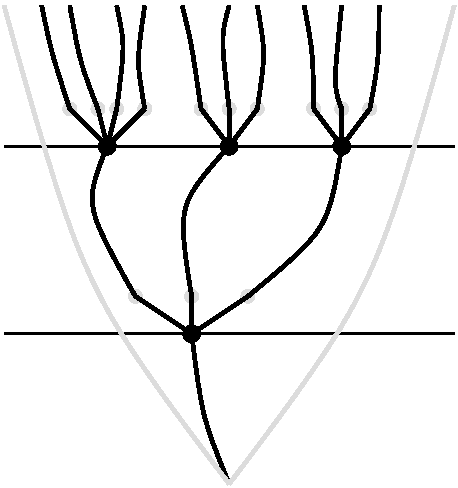
\includegraphics[scale=0.5]{figures/strongTree.pdf}
	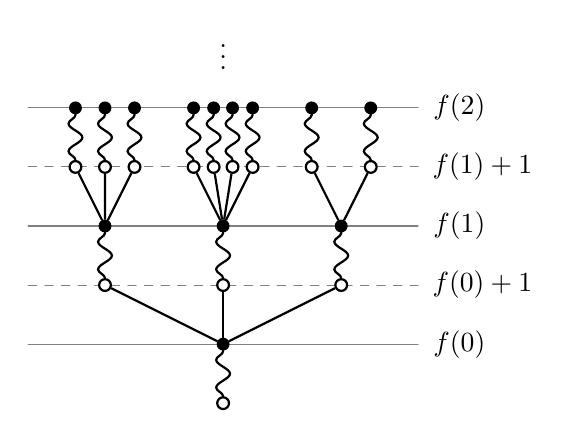
\begin{tikzpicture}[scale=1.5,font=\normalsize]
		\tikzset{
		empty node/.style={circle,inner sep=0,fill=none},
		solid node/.style={circle,draw,inner sep=1.5,fill=black},
		hollow node/.style={circle,draw,thick,inner sep=1.5,fill=white}
		}
		\tikzset{snake it/.style={decorate, decoration=snake, line cap=round}}
		\tikzset{gray line/.style={line cap=round,color=gray}}
		\tikzset{thin line/.style={line cap=round}}
		\draw[color=gray,-,thin line] (-1.65,0.5) to (1.65,0.5);
		\draw[color=gray,-,thin line] (-1.65,1.5) to (1.65,1.5);
		\draw[color=gray,-,thin line] (-1.65,2.5) to (1.65,2.5);
		\draw[color=gray,-,thin line,dash pattern={on 3pt off 3pt}] (-1.65,1) to (1.65,1);
		\draw[color=gray,-,thin line,dash pattern={on 3pt off 3pt}] (-1.65,2) to (1.65,2);
		\node(a)[hollow node] at (0,0) {};
		\node(b)[solid node] at (0,0.5) {};
		\node(b0)[hollow node] at (-1,1) {};
		\node(b1)[hollow node] at (0,1) {};
		\node(b2)[hollow node] at (1,1) {};
		\node(b0')[solid node] at (-1,1.5) {};
		\node(b1')[solid node] at (0,1.5) {};
		\node(b2')[solid node] at (1,1.5) {};
		\node(b0'0)[hollow node] at (-1.25,2) {};
		\node(b0'1)[hollow node] at (-1,2) {};
		\node(b0'2)[hollow node] at (-0.75,2) {};
		\node(b1'0)[hollow node] at (-0.25,2) {};
		\node(b1'1)[hollow node] at (-0.08,2) {};
		\node(b1'2)[hollow node] at (0.08,2) {};
		\node(b1'3)[hollow node] at (0.25,2) {};
		\node(b2'0)[hollow node] at (0.75,2) {};
		\node(b2'1)[hollow node] at (1.25,2) {};
		\node(dots)[empty node] at (0,3) {$\vdots$};
		\node[empty node] at (2,0.5) {$f(0)$};
		\node[align=flush left] at (2,1) {~~~~~$f(0)+1$};
		\node[empty node] at (2,1.5) {$f(1)$};
		\node[align=flush left] at (2,2) {~~~~~$f(1)+1$};
		\node[align=flush left] at (2,2.5) {$f(2)$};

		\node(b0'0')[solid node] at (-1.25,2.5) {};
		\node(b0'1')[solid node] at (-1,2.5) {};
		\node(b0'2')[solid node] at (-0.75,2.5) {};
		\node(b1'0')[solid node] at (-0.25,2.5) {};
		\node(b1'1')[solid node] at (-0.08,2.5) {};
		\node(b1'2')[solid node] at (0.08,2.5) {};
		\node(b1'3')[solid node] at (0.25,2.5) {};
		\node(b2'0')[solid node] at (0.75,2.5) {};
		\node(b2'1')[solid node] at (1.25,2.5) {};

		\draw[thick,snake it] (a) to (b);
		\draw[thick,-] (b) to (b0);
		\draw[thick,-] (b) to (b1);
		\draw[thick,-] (b) to (b2);
		\draw[thick,snake it] (b0) to (b0');
		\draw[thick,snake it] (b1) to (b1');
		\draw[thick,snake it] (b2) to (b2');
		\draw[thick,-] (b0') to (b0'0);
		\draw[thick,-] (b0') to (b0'1);
		\draw[thick,-] (b0') to (b0'2);
		\draw[thick,-] (b1') to (b1'0);
		\draw[thick,-] (b1') to (b1'1);
		\draw[thick,-] (b1') to (b1'2);
		\draw[thick,-] (b1') to (b1'3);
		\draw[thick,-] (b2') to (b2'0);
		\draw[thick,-] (b2') to (b2'1);
		\draw[thick,snake it] (b0'0) to (b0'0');
		\draw[thick,snake it] (b0'1) to (b0'1');
		\draw[thick,snake it] (b0'2) to (b0'2');
		\draw[thick,snake it] (b1'0) to (b1'0');
		\draw[thick,snake it] (b1'1) to (b1'1');
		\draw[thick,snake it] (b1'2) to (b1'2');
		\draw[thick,snake it] (b1'3) to (b1'3');
		\draw[thick,snake it] (b2'0) to (b2'0');
		\draw[thick,snake it] (b2'1) to (b2'1');
		%\draw[gray line,out=20,in=-90] (a) to (2,3);
		%\draw[gray line,out=170,in=-90] (a) to (-2,3);
	\end{tikzpicture}
  	\caption{A strong subtree $S$ of a tree $T$, with level function $f$. The circles represent nodes in $T$; the solid circles in $S$, the hollow circles are in $T \setminus S$. The levels of $S$ are included in the level{s} of $T$; solid gray horizontal lines represent levels in $S$, dashed gray horizontal lines levels in $T \setminus S$. A node connected to another below it by a straight black line denotes a direct extension in $T$. Wavy lines indicate omitted (skipped over) portions of $T$. Note that all branchings are preserved: a nodes in $S$ has the same number of direct extensions in $S$ as in $T$.}
  	\label{fig:strong-subtree}
\end{figure}

\section{Forests and products of trees}\label{sec:bkg_forests}

As mentioned above, in order to study the proof of Milliken's tree theorem we will need to examine the Halpern-La\"{u}chli theorem, whose statements requires us to consider multiple trees in parallel.

\begin{definition}\label{def:forest}
	A \emph{forest}\index{forest} is a non-empty subset $X$ of $\omega^{<\omega}$ such that if a pair of nodes $\sigma,\tau \in X$ has a common initial segment in $X$ then also $\sigma \meet \tau \in X$.
%A \emph{forest} is a non-empty set $X \subseteq \omega^{<\omega}$ such that if a pair of nodes $\sigma, \tau \in X$ admits a common prefix in $X$, then $\sigma \meet \tau \in X$. A node $\sigma \in X$ is a \emph{root} of $X$ if it has no prefix in $X$.   We write $X(n)$ for the set of nodes of $X$ such that $|\{\tau\in X:\tau\prec\sigma\}|=n$. The \emph{level} of a node is the number $n$ such that $\sigma\in X(n)$. A node $\sigma\in X(n)$ is \emph{$k$-branching} iff $\sigma$ has exactly $k$ pairwise incomparable extensions in $X(n+1)$. A \emph{leaf} is a 0-branching node. % The \emph{meet in $X$} of two nodes $\sigma,\tau\in X$, if it exists, is the common predecessor of $\sigma$ and $\tau$ with the largest level in $X$, written $\sigma\meet_X\tau$.
\end{definition}

Since every pair of nodes in a tree has at least one common initial segment (the root), it is clear that every tree is a forest. Indeed, the following is easy to see: $X \subseteq \baire$ is a forest if and only if it is a union of disjoint trees. For this reason, we refer to the elements of a forest as nodes, and lift all other terminology from trees to forests. For definiteness, we make this explicit in the following definition.

\begin{definition}
	Let $X$ be a forest.
	\begin{enumerate}
		\item A \emph{root}\index{forest!root}\index{root!forest} of $X$ is any $\rho \in T$ having no proper initial segment in $X$. The set of all roots of $X$ is denoted by $\roots(X)$\index{$\roots(X)$}.
		\item The \emph{level}\index{node!level}\index{level} of $\sigma \in X$ is $|\{ \tau \in X: \tau \prec \sigma\}|$. We say $\sigma$ is \emph{at} this level in $X$.
		\item For $n \in \NN$, $X(n)$ denotes the set of all $\sigma \in X$ at level $n$ in $X$.
		\item The \emph{height}\index{forest!height}\index{height!forest} of $X$ is the least ordinal $\alpha$ larger than the level of every $\sigma \in X$.
		\item If $\sigma,\tau \in X$ with $\sigma \prec \tau$ and there is no $\tau' \in X$ with $\sigma \prec \tau' \prec \tau$, then $\tau$ is a \emph{direct extension}\index{direct extension!forest}\index{node!direct extension} of $\sigma$ in $X$.
		\item For $k \in \omega$, a node $\sigma \in X$ is \emph{$k$-branching} in $X$ if it has exactly $k$ many direct extensions in $X$.
		\item A node $\sigma \in X$ is a \emph{leaf}\index{leaf}\index{node!leaf} of $X$ if it is $0$-branching. The set of leaves of $X$ is denoted $\leaves(X)$.
	\end{enumerate}
\end{definition}

\noindent Thus, a forest $X$ is a tree if and only if $\roots(X)$ is a singleton. The height of $X$ is the maximum of the heights of the disjoint trees that comprise it.

Given a forest $X$ and a node $\sigma \in X$, we let $X \uh \sigma = \{ \tau \in X: \tau \succeq \sigma \}$. In particular, whenever $\sigma \in X$ we have that $X \uh \sigma$ is a tree with root $\sigma$.

\begin{definition}
  A forest $Y$ of height $\alpha \leq \omega$ is a \emph{strong subforest}\index{forest!strong subforest}\index{strong subforest} of a forest $X$ if it satisfies the following two properties:
  \begin{enumerate}
  \item there exists a function $f: \alpha \to \omega$, called a \emph{level function}, such that for all $n \leq \alpha$, if $\sigma \in X(n)$ then $\sigma \in X(f(n))$;
  %\item There exists a function $f:\om\to\om$ mapping levels to levels, such that $\forall n\forall \sigma\in Y(n), \sigma\in X(f(n))$.  We shall later refer to this function as the \emph{level function}.
  \item for all $k$, a node in $Y$ which is not at level $\alpha$ in $Y$ is $k$-branching in $Y$ if and only if it is $k$-branching in $X$.
  %\item If $\sigma\in Y\cap X(f(n))$, then for every $\tau\in X(f(n)+1)$ extending $\sigma$, there exists a unique $\rho\in Y\cap X(f(n+1))$ extending $\tau$.
  \end{enumerate}
\end{definition}

\noindent Given a forest $X$ and an $\alpha \leq \omega$, we let $\Subtree{\alpha}{X}$\index{$\Subtree{\alpha}{}$!forest} be the collection of all strong subforests of $X$ of height $\alpha$. We also add the following slightly more general definition.

\begin{definition}
	For each $d \geq 1$, if $T_0,\ldots,T_{d-1}$ are trees then $\Subtree{\alpha}{T_0,\dots, T_{d-1}}$\index{$\Subtree{\alpha}{}$!product of trees} for $\alpha \leq \omega$ is the collection of all tuples $(S_0,\ldots,S_{d-1})$ such that for each $i < d$ we have $S_i \in \Subtree{\alpha}{T_i}$, witnessed by one and the same level function. In addition, $\Subtree{<\alpha}{T_0,\dots, T_{d-1}}$\index{$\Subtree{<\alpha}{}$} denotes $\bigcup_{n < \alpha} \Subtree{n}{T_0,\dots, T_{d-1}}$.
\end{definition}

\noindent Thus, if $X = \bigcup_{i < d} T_i$, where $T_0,\ldots,T_{d-1}$ are disjoint trees, then $\Subtree{\alpha}{X} = \Subtree{\alpha}{T_0,\ldots,T_{d-1}}$. However, the preceding definition applies to arbitrary trees $T_0,\ldots,T_{d-1}$, disjoint or not.

We include one final definition, which is standard in other investigations of Milliken's tree theorem and will be important to us going forward.

\begin{definition}
	Fix $m \geq 1$.
	\begin{enumerate}
		\item For a forest $X$ and node $\sigma \in X$, a subset $P$ of $X$ is \emph{$m$-$\sigma$-dense}\index{$m$-$\sigma$-dense}\index{dense!subset}\index{dense!$m$-$\sigma$-dense} if every $\tau \in X(m)$ that extends $\sigma$ has an extension in $P$.
		\item For forests $X_0,\ldots,X_{d-1}$ and tuple $\pi = (\sigma_0,\ldots,\sigma_{d-1}) \in \bigcup_{n} X_0(n) \times \cdots \times X_{d-1}(n)$, a subset $P$ of $X_0 \times \cdots \times X_{d-1}$ is an \emph{$m$-$\pi$-dense matrix}\index{dense!matrix}\index{$m$-$\pi$-dense matrix} if $P = P_0 \times \cdots \times P_{d-1}$ where $P_i$ is an $m$-$\sigma_i$-dense subset of $X_i$, for each $i < d$.
	\end{enumerate}
\end{definition}

\noindent We will of course only be interested in the case where $m$ is larger than the level of $\sigma$ in $X$, respectively, of the (common) level in $X_i$ of each of the entries $\sigma_i$ of $\pi$. In the latter case, we will call this common level the \emph{level of $\pi$} in $X$.

The main point in item 2 above is that if $P$ is an $m$-$\pi$-dense matrix then for every $\tau_i \in X_i(m)$ that extends $\sigma_i$ we can find a $\rho_i$ such that $(\rho_0,\ldots,\rho_{d-1}) \in P$, and the latter is true for every choice of possible $\rho_i$. Note that the $\rho_i$ do not have to be at the same level in their respective forests. Also, notice that the $X_i$ need not be disjoint, and so their union need not be itself a forest.

\section{Statements of theorems}\label{sec:bkg_stmts}

In this section, we can finally define Milliken's tree theorem and its combinatorial variants that we will investigate in \Cref{sect:hl-theorem,sect:milliken-theorem}, as well as the various application of Milliken's tree theorem that we will discuss in \Cref{sec:devlin,sec:radomain,sec:GenCHMTT}.

\begin{theorem}[Milliken's tree theorem]\label{th:milliken-theorem}\index{tree theorem!Milliken's tree theorem|textbf}\index{theorem!Milliken's tree theorem|textbf}\index{Milliken's tree theorem|textbf}
	Let $T$ be an infinite tree with no leaves. For all $n,k \geq 1$ and all $f:\Subtree{n}{T} \to k$ there is an $S \in \Subtree{\omega}{T}$ such that $f$ is constant on $\Subtree{n}{S}$.
\end{theorem}

By analogy with Ramsey's theorem, we will break this statement up into sub-statements, in this case according to the height of the subtrees being colored. Thus, we define the following:

\begin{statement}\index{statement!$\MT n{}$|textbf}\index{Milliken's tree theorem!$\MT n{}$|textbf}
For all $n \geq 1$, $\MT n{}$ is the restriction of Milliken's tree theorem to colorings to strong subtrees of height~$n$.
\end{statement}

\noindent We will sometimes also refer to $\MT n{}$ as \emph{Milliken's tree theorem for height $n$} in the sequel. From the computability-theoretic point of view, we will regard an instance of $\MT n{}$ as being a tuple $\seq{T,b,f,k}$, where $T$ is an infinite $b$-bounded tree with no leaves, and $f$ is a map $\Subtree{n}{T} \to k$. In effect, this means all computable instances of $\MT n {}$ are computably bounded.

As discussed in the introduction, the next theorem is the analogue of the pigeonhole principle in the proof of Milliken's tree theorem.

\begin{theorem}[Halpern-La\"{u}chli theorem]\label{th:strong-hl}\index{tree theorem!Halpern-La\"{u}chli theorem|textbf}\index{theorem!Halpern-La\"{u}chli theorem|textbf}\index{Halpern-La\"{u}chli theorem|textbf}
	Let $T_0,\ldots,T_{d-1}$ be infinite trees with no leaves. For all $k \geq 1$ and all $f: \bigcup_{n} T_0(n) \times \cdots \times T_{d-1}(n) \to k$ there exists $(S_0,\ldots,S_{d-1}) \in \Subtree{\omega}{T_0,\ldots,T_{d-1}}$ such that $f$ is constant on $\bigcup_{n} S_0(n) \times \cdots \times S_{d-1}(n)$.
\end{theorem}

\noindent Again, one would naturally expect $\MT 1{}$ to play this role, so the need for the Halpern-La\"{u}chli theorem is not a priori obvious. In fact, the original paper~\cite{Milliken1979RTforTrees} that introduced what we now call Milliken's tree theorem actually proved a version for products that looks much more like the ``general case'' of the Halpern-La\"{u}chli theorem. In many ways, this is really the more natural result, and Milliken's tree theorem is merely a restriction that suffices for most applications.

% following theorem was proven by Milliken in~\cite{Milliken1979RTforTrees}.

\begin{theorem}[Product version of Milliken's tree theorem]\label{th:product-MTT}\index{tree theorem!Milliken's tree theorem for product|textbf}\index{theorem!Milliken's tree theorem for product|textbf}\index{Milliken's tree theorem!product version|textbf}
	Let $T_0,\ldots,T_{d-1}$ be infinite trees with no leaves. For all $n,k \geq 1$ and all $f: \Subtree{n}{T_0,\ldots,T_{d-1}} \to k$ there exists $(S_0,\ldots,S_{d-1}) \in \Subtree{\omega}{T_0,\ldots,T_{d-1}}$ such that $f$ is constant on $\Subtree{n}{S_0,\ldots,S_{d-1}}$.
\end{theorem}

\begin{statement}\index{statement!$\PMT n{}$|textbf}\index{Milliken's tree theorem!$\PMT n{}$|textbf}
  For all $n \geq 1$, $\PMT n{}$ is the restriction of the product version of Milliken's tree theorem for height $n$.
\end{statement}

\noindent The Halpern-La\"{u}chli theorem is exactly $\PMT 1{}$, since for all $T_0,\ldots,T_{d-1}$ we have
\[
	\Subtree{1}{T_0,\dots, T_{d-1}}=\bigcup_{n}T_0(n)\times\dots\times T_{d-1}(n).
\]
In our analysis, we will regard an instance of $\PMT n{}$ as a tuple
\[
	\seq{d,T_0,\ldots,T_{d-1},b,f,k},
\]
where the $T_i$ are infinite $b$-bounded trees with no leaves, and $f$ is a map $\Subtree{n}{T_0,\ldots,T_{d-1}} \to k$.

We now state some further applications of Milliken's tree theorem, which concern various structures besides trees. Each of these structures will be countable and, unless otherwise stated, infinite, and will have a countable, relational underlying language. For a finite substructure $\mathcal{A}$ of a structure $\mathcal{B}$, let %$[\mathcal{B}]^\mathcal{A}$
$\mathcal{B} \choose \mathcal{A}$ \index{$\mathcal{B} \choose \mathcal{A}$}
denote the set of (isomorphic) copies of $\mathcal{A}$ contained in $\mathcal{B}$. Recall also that if $X$ is a set and $n$ is a positive integer then $[X]^n$ \index{$[X]^n$} denotes the set of $n$-element subsets of $X$. In particular, if $B$ is the domain of $\mathcal{B}$, then each element of $[B]^n$ may be regarded as a substructure of $\mathcal{B}$ by restriction since the language of $\mathcal{B}$ is relational. (In general, however, $[B]^n$ need not equal $\mathcal{B} \choose \mathcal{A}$ for any one $\mathcal{A}$.) When convenient, we may also write $[\mathcal{B}]^n$ for $[B]^n$.

The first application of Milliken's tree theorem we consider is \emph{Devlin's theorem}, also called \emph{Devlin's second theorem}, e.g., in \cite{Todorcevic2010Ramsey}, Chapter 6.
\begin{theorem}[Devlin's theorem]\index{theorem!Devlin's theorem|textbf}\index{Devlin's theorem|textbf}
	For every $n \geq 1$ there exists $\ell \geq 1$ such that for every $k \geq 1$ and every $f: [\mathbb{Q}]^n \to k$ there is a dense suborder $S$ of $\mathbb{Q}$ with no endpoints satisfying $|f ([S]^n)| \leq \ell$.
\end{theorem}

\noindent The key here is that the bound $\ell$ does not depend on $k$ or the particular coloring, but only on $n$. As an instance-solution problem, we will study Devlin's theorem in the following form:

\begin{statement}\index{statement!$\DT n{k,\ell}$|textbf}
  For all $n, k, \ell \geq 1$, $\DT{n}{k,\ell}$ is the assertion that for every $f: [\mathbb Q]^n \to k$ there is a dense suborder $S$ of $\mathbb{Q}$ with no endpoints satisfying $|f ([S]^n)| \leq \ell$.
\end{statement}

\noindent Note that $\DT{n}{k,\ell}$ is merely a formal statement, not a necessarily a true theorem for all possible $n$, $k$, and $\ell$. For example, it is easy to see that $\DT{1}{k,1}$ is true for all $k$. However, $\DT{2}{2,1}$ is false. 
%\noindent It is easy to see that if $n = 1$ then we can take $\ell = 1$. However, for $n \geq 2$, this is no longer the case, so Devlin's theorem is not a direct extension of Ramsey's theorem.
To see this, let $(q_n)_{n\in\Nb}$ be an enumeration of the rationals, and define $f: [\mathbb Q]^2\to 2$ by letting $f(q_n, q_m) = 0$ if $q_n<q_m\iff n<m$, and $f(q_n, q_m) = 1$ otherwise. Then it is readily seen that every subset $S\subseteq\mathbb Q$ of order-type $\mathbb Q$ (or even $\mathbb Z$) must contain pairs of both colors under $f$. For $n = 2$, this situation turns out to be as bad as it can be, as $\DT{2}{k,2}$ is true for all $k$. This fact was originally observed by Galvin (unpublished). For general $n$, the corresponding $\ell$ values were obtained by Devlin \cite[Chapter 4]{Devlin1980}.

The second application we consider concerns graph colorings. We use $\mathcal{G}$ as generic notation for a graph, and unless otherwise specified, assume the set of vertices of $\mathcal{G}$ is $G$, and the set of edges, $E$. For $x,y \in G$, we write $xEy$ if $(x,y) \in E$ and $\lnot x E y$ if $(x,y) \notin E$. The graph $\mathcal{G}$ is a \emph{Rado graph} (or \emph{random graph}) \index{graph!Rado} \index{graph!random|see{Rado}} \index{Rado Graph} if for every two disjoint finite sets of vertices $F_0,F_1 \subseteq G$ there exists $x \in G$ such that $xEy$ for all $y \in F_0$ and $\lnot x E y$ for all $y \in F_1$. Such a graph is, in particular, universal, containing every finite graph as an induced subgraph. All Rado graphs are isomorphic by the standard back and forth construction, so we usually speak just of \emph{the} Rado graph, and assume we have fixed a canonical computable representative of it, denoted by $\mathcal{R}$. The principle of interest to us is following, which we will call the \emph{Rado graph theorem} here for definiteness.
\begin{theorem}[Rado graph theorem]\index{theorem!Rado graph theorem}\index{Rado graph theorem}
	For every finite graph $\mathcal{G}$ there exists $\ell \geq 1$ such that for every $k \geq 1$ and every $f: {\mathcal{R} \choose \mathcal{G}} \to k$ there is an isomorphic subgraph $\mathcal{R}'$ of $\mathcal{R}$ satisfying $|f'' {\mathcal{R}' \choose \mathcal{G}}| \leq \ell$.
\end{theorem}

Again, the bound $\ell$ does not depend on $k$, but only, in this case, on the particular subgraph $\mathcal{G}$. The precise bounds here were obtained by Sauer \cite{Sauer2006} and Laflamme, Sauer, and Vuksanovic \cite{LSV2006}. The result shares much in common with Devlin's theorem, as we will see further below. Both results are well-known consequences of Milliken's theorem. (See, e.g., Todorcevic \cite{Todorcevic2010Ramsey}, Theorems 6.23 and 6.25 for direct proofs.) We give a more effective proof of the Rado graph theorem from Milliken's tree theorem in \Cref{subsect:rado-from-mtt}.

We will investigate the Rado graph theorem in the following two forms.

\begin{statement}\index{statement!$\RG^\mathcal{G}_{k,\ell}$}
For all finite graphs $\mathcal{G}$ and all $k,\ell \geq 1$, $\RG^\mathcal{G}_{k,\ell}$ is the assertion that for every coloring $f: {\mathcal{R} \choose \mathcal{G}} \to k$, there is an isomorphic subgraph $\mathcal{R}'$ of $\mathcal{R}$ satisfying $|f''{\mathcal{R}' \choose \mathcal{G}}| \leq \ell$.
\end{statement}

\begin{statement}\index{statement!$\RG^n_{k,\ell}$}
For all $n,k,\ell \geq 1$, $\RG^n_{k,\ell}$ is the assertion that for every coloring $f: [\mathcal{R}]^n \to k$, there is an isomorphic subgraph $\mathcal{R}'$ of $\mathcal{R}$ satisfying $|f''[\mathcal{R}']^n| \leq \ell$.
\end{statement}

\noindent Since there are, up to isomorphism, only finitely many graphs $G$ of a given finite size, we immediately get the implication
\[
	(\forall \mathcal{G})(\exists \ell)(\forall k)[\RG^\mathcal{G}_{k,\ell}] \to (\forall n)(\exists \ell)(\forall k)[\RG^n_{k,\ell}].
\]

The final application we look at, unlike the previous two, is not a familiar one in set theory. However, it has been studied extensively in computable combinatorics and reverse mathematics (see, e.g., \cite{Chong2019Strengtha, Chong2019Strengthb, Chong2019Strengthc, Dzhafarov2017Coloring, Patey2016strength} for some very recent papers). This is the tree theorem of Chubb, Hirst, and McNicholl \cite{Chubb2009Reverse}, which we will refer to as the \emph{Chubb-Hirst-McNicholl (CHM) tree theorem} in this monograph, to avoid confusion with Milliken's tree theorem. The CHM tree theorem concerns a weaker structure of tree than in Definition \ref{def:trees}, where we do not insist on being closed under meets. A tree is thus any subset of $2^{<\omega}$ with a root. The theorem asserts the existence, for every finite coloring of the $n$-tuples of \emph{comparable} nodes of $\cantor$, of an infinite monochromatic perfect subtree in this weaker sense. The restriction to comparable nodes comes from wanting to extend Ramsey's theorem to these ``weak'' trees. And indeed, as in Devlin's theorem, it is easy to devise a coloring of arbitrary tuples of nodes here where no monochromatic solution exists (e.g., consider coloring all comparable pairs of strings $0$, and all incomparable pairs of strings $1$). As it turns out, this restriction loses a great deal of combinatorial structure, which becomes apparent if we look not for monochromatic solutions, but merely for bounds on the numbers of colors used in a solution. It is this generalization of the CHM tree theorem that we investigate.

\begin{theorem}[Generalized CHM tree theorem]\index{theorem!generalized CHM tree theorem|textbf}\index{tree theorem!generalized CHM tree theorem|textbf}\index{theorem!Chubb, Hirst, McNicholl|see{generalized CHM tree theorem}}\index{generalized CHM tree theorem|textbf}
	For every $n \geq 1$ there exists $\ell \geq 1$ such that for every $k \geq 1$ and every $f: [2^{<\omega}]^n \to k$ there is an $S \subseteq 2^{<\omega}$ such that $(S,\preceq)$ is isomorphic to $(2^{<\omega},\preceq)$ and $|f ([S]^n)| \leq \ell$.
\end{theorem}

\begin{statement}\index{statement!$\CHMTT^n_{k,\ell}$}
	For all $n,k,\ell \geq 1$,	$\CHMTT^n_{k,\ell}$ is the assertion that for every $f: [2^{<\omega}]^n \to k$ there is an $S \subseteq 2^{<\omega}$ such that $(S,\preceq)$ is isomorphic to $(2^{<\omega},\preceq)$ and $|f ([S]^n)| \leq \ell$.
\end{statement}


\noindent As with the previous two principles, the CHM tree theorem is a consequence of Milliken's tree theorem. We include a proof in Theorem \ref{th:strong_gen_treeth} below.

\section{Big Ramsey degrees and structures}\label{sec:bigRamsey}

Though we will study each of Devlin's theorem, the Rado graph theorem, and the CHM tree theorem separately and in its own right, we mention a common framework within which all three can be presented, and which better highlights some of the main similarities between the three. Some of the terminology here will also be convenient in our discussions later on.

All three principles can be stated more succinctly using the concept of big Ramsey degrees, which we now review. Recall that if $\mathcal{B}$ is an infinite structure and $\mathcal{A}$ is a finite substructure of $\mathcal{B}$, then for positive numbers $\ell \leq k$ the notation
\[
\mathcal{B} \to (\mathcal{B})^{\mathcal{A}}_{k,\ell}
\]
means that for every coloring $f: {\mathcal{B} \choose \mathcal{A}} \to k$ there exists an isomorphic substructure $\mathcal{B}'$ of $\mathcal{B}$ such that $|f '' {\mathcal{B}' \choose \mathcal{A}}| \leq \ell$. The following terminology is standard in structural Ramsey theory.

\begin{definition}\label{D:bigRamsey}
	Let $\mathcal{B}$ be a structure.
	\begin{itemize}
		\item For a finite substructure $\mathcal{A}$ of $\mathcal{B}$, the \emph{big Ramsey degree of $\mathcal{A}$ in $\mathcal{B}$} \index{big Ramsey degree} \index{Ramsey!big degree} is the least number $\ell \in \omega$, if it exists, such that $\mathcal{B} \to (\mathcal{B})^\mathcal{A}_{k,\ell}$ for all $k \in \omega$, in which case we say that the big Ramsey degree of $\mathcal{A}$ is \emph{finite}.
		\item We say that a structure \emph{$\mathcal{B}$ has finite big Ramsey degrees} \index{big Ramsey degree!finite} if, for every finite substructure $\mathcal{A}$ of $\mathcal{B}$ has finite big Ramsey degree.
	\end{itemize}
\end{definition}

\noindent In the parlance of this definition, then, the Rado graph theorem is simply the assertion that the Rado graph has finite big Ramsey degrees. Similarly, Devlin's theorem is the assertion that $(\mathbb{Q},<)$ has finite big Ramsey degrees, since up to isomorphism $(\mathbb{Q},<)$ has exactly one finite substructure $\mathcal{A}$ of each size $n \geq 1$, and so ${(\mathbb{Q},<) \choose \mathcal{A}} = [\mathbb{Q}]^n$. For the generalized CHM tree theorem the situation is slightly different. While $(2^{<\omega},\preceq)$ can have more than one non-isomorphic substructure of a given finite size, it still has only finitely many. Thus, the generalized CHM tree theorem is equivalent to the statement that $(2^{<\omega},\preceq)$ has finite big Ramsey degrees.

The bounds $\ell$ in each of Devlin's theorem, the Rado graph theorem, and the generalized CHM tree theorem are not determined purely by properties of the underlying structures. For example, even though $\mathbb{Q}$ has only one substructure of size $2$ up to isomorphism, we saw that we could differentiate two \emph{types} of substructure of size $2$ by enriching the structure by an enumeration of the domain. Enrichments of this kind play an important role in these computations, since they can be taken into account in designing colorings with a certain number of unavoidable colors.

A precise formalization of the concept of ``enrichment'' is given by Zucker \cite{Zucker-2019}.

\begin{definition}[Zucker \cite{Zucker-2019}, Definition 1.3]\label{def:big-ramsey-structure}\index{big Ramsey structure}\index{Ramsey!big structure}
	Let $\mathcal{B}$ be a structure in a language $\mathscr{L}$. A \emph{big Ramsey structure for $\mathcal{B}$} is a structure $\hat{\mathcal{B}}$ in a language $\hat{\mathscr{L}}$ satisfying the following properties:
	\begin{enumerate}
		\item $\mathscr{L} \subseteq \hat{\mathscr{L}}$;
		\item the restriction of $\hat{\mathcal{B}}$ to $\mathscr{L}$ is $\mathcal{B}$;
		\item for every finite substructure $\mathcal{A}$ of $\mathcal{B}$ there is a number $t_{\hat{\mathcal{B}}}(\mathcal{A})$ such that, up to isomorphism, there are exactly $t_{\hat{\mathcal{B}}}(\mathcal{A})$ many different substructures $\hat{\mathcal{A}}$ of $\hat{\mathcal{B}}$ whose restriction to $\mathscr{L}$ is a copy of $\mathcal{A}$;
		\item every finite substructure $\mathcal{A}$ of $\mathcal{B}$ has big Ramsey degree equal to $t_{\hat{\mathcal{B}}}(\mathcal{A})$;
		\item for every finite substructure $\mathcal{A}$ of $\mathcal{B}$ and choice $\hat{\mathcal{A}}_0,\ldots,\hat{\mathcal{A}}_{t_{\hat{\mathcal{B}}}(\mathcal{A})-1}$ of substructures of $\hat{\mathcal{B}}$ as in property 3, the coloring $f: {\mathcal{B} \choose \mathcal{A}} \to t_{\hat{\mathcal{B}}}(\mathcal{A})$ mapping each copy of $\mathcal{A}'$ of $\mathcal{A}$ in $\mathcal{B}$ to the unique $i < t_{\hat{\mathcal{B}}}(\mathcal{A})$ such that $\mathcal{A}'$, viewed as a substructure of $\hat{\mathcal{B}}$ by restriction, is isomorphic to $\hat{\mathcal{A}}_i$ witnesses that the big Ramsey degree of $\mathcal{A}$ in $\mathcal{B}$ is at least $t_{\hat{\mathcal{B}}}(\mathcal{A})$.
	\end{enumerate}
\end{definition}

\noindent The idea here is that for every finite substructure $\mathcal{A}$ of $\mathcal{B}$, the substructures $\hat{\mathcal{A}}_0,\ldots,\hat{\mathcal{A}}_{t_{\hat{\mathcal{B}}}(\mathcal{A})}$ of $\hat{\mathcal{B}}$ satisfying property 3 represent all recognizable or describable types of the copies of $\mathcal{A}$ in $\mathcal{B}$, and the additional structure of $\hat{\mathcal{B}}$ facilitates these descriptions. In the literature, these instances are called more specifically \emph{embedding types} or \emph{Devlin types} based on the specific structure $\mathcal{B}$.

Zucker \cite[Theorem 7.1]{Zucker-2019} provides some sufficient (and somewhat technical) conditions for a structure to admit a big Ramsey structure. For our purposes here, it is enough to know that each of $(\mathbb{Q},\leq)$, the Rado graph, and $(2^{<\omega},\preceq)$ does. We will study the big Ramsey structure of the Rado graph in detail (see also \cite{Zucker-2019}, Section 6.3), and we will carefully develop the appropriate notion of type in the sense of the big Ramsey structure for the generalized CHM tree theorem. For an account of a big Ramsey structure for $(\mathbb{Q},\leq)$, see \cite[Section 6.2]{Zucker-2019}.


%%% Local Variables:
%%% mode: latex
%%% TeX-master: "../embryon"
%%% End:
